% =====================================================================
%  MCMP117 -- Fundamentals of Operating Systems
%  Week 4 Course Notes: Threads & CPU Scheduling Basics
%  Compile with XeLaTeX (twice):  xelatex MCMP117_Week4_Notes.tex
%  Needs ./figures/ and the ../code/ folder.
% =====================================================================
\documentclass[11pt,a4paper]{article}
\newcommand{\weeknum}{4}
% ---------- Page & fonts ---------------------------------------------
\usepackage[a4paper,margin=2.3cm,headheight=15pt]{geometry}
\usepackage{fontspec}
\IfFontExistsTF{Calibri}{\setmainfont{Calibri}}{\setmainfont{Carlito}}
\IfFontExistsTF{Cambria}{\newfontfamily\headfont{Cambria}}{\newfontfamily\headfont{Caladea}}
\IfFontExistsTF{Consolas}{\setmonofont[Scale=0.95]{Consolas}}{\setmonofont[Scale=0.88]{DejaVu Sans Mono}}
\usepackage{amsmath,amssymb}
\usepackage{microtype}
\linespread{1.12}
\setlength{\parskip}{0.55em}
\setlength{\parindent}{0pt}

% ---------- Colours (course design system) ----------------------------
\usepackage{xcolor}
\definecolor{dark}{HTML}{212121}
\definecolor{charcoal}{HTML}{36454F}
\definecolor{slate}{HTML}{50808E}
\definecolor{mint}{HTML}{02C39A}
\definecolor{mintdeep}{HTML}{028090}
\definecolor{light}{HTML}{F2F2F2}
\definecolor{muted}{HTML}{6B7679}

% ---------- Packages ---------------------------------------------------
\usepackage{graphicx}
\usepackage{float}
\usepackage{needspace}
\graphicspath{{figures/}}
\usepackage[font=small,labelfont={bf,color=mintdeep},justification=centering]{caption}
\usepackage{booktabs,longtable,array,tabularx}
\usepackage{enumitem}
\setlist{itemsep=0.25em,topsep=0.3em}
\usepackage{tikz}
\usetikzlibrary{arrows.meta,positioning,calc,shapes.geometric}
\usepackage{pgfplots}
\pgfplotsset{compat=1.17}
\usepackage[most]{tcolorbox}
\usepackage{titlesec}
\usepackage{fancyhdr}
\usepackage{xurl}
\usepackage[colorlinks=true,linkcolor=mintdeep,urlcolor=mintdeep,citecolor=mintdeep]{hyperref}

% ---------- Headings ----------------------------------------------------
\titleformat{\section}{\headfont\Large\bfseries\color{charcoal}}{\color{mint}\thesection}{0.7em}{}
\titleformat{\subsection}{\headfont\large\bfseries\color{charcoal}}{\color{mintdeep}\thesubsection}{0.6em}{}
\titleformat{\subsubsection}{\headfont\normalsize\bfseries\color{mintdeep}}{}{0em}{}
\titlespacing*{\section}{0pt}{1.6em}{0.6em}
\titlespacing*{\subsection}{0pt}{1.2em}{0.4em}

% ---------- Header / footer -----------------------------------------------
\pagestyle{fancy}
\fancyhf{}
\fancyhead[L]{\small\color{muted}MCMP117 --- Fundamentals of Operating Systems}
\fancyhead[R]{\small\color{muted}Week \weeknum{} Notes}
\fancyfoot[C]{\small\color{muted}\thepage}
\renewcommand{\headrulewidth}{0pt}

% ---------- Boxes ---------------------------------------------------------
\newtcolorbox{keyidea}[1][Key idea]{enhanced,breakable,colback=charcoal,colframe=charcoal,
  coltext=white,fonttitle=\headfont\bfseries\color{mint},title={#1},
  attach title to upper={\par\smallskip},boxrule=0pt,arc=3pt,left=10pt,right=10pt,top=8pt,bottom=8pt}
\newtcolorbox{example}[1][Worked example]{enhanced,colback=light,colframe=light,
  fonttitle=\headfont\bfseries\color{mintdeep},title={#1},attach title to upper={\par\smallskip},
  boxrule=0pt,arc=3pt,left=10pt,right=10pt,top=8pt,bottom=8pt}
\newtcolorbox{tryit}[1][Try it yourself]{enhanced,breakable,colback=white,colframe=mint,
  fonttitle=\headfont\bfseries\color{mintdeep},title={#1},attach title to upper={\par\smallskip},
  boxrule=0.8pt,arc=3pt,left=10pt,right=10pt,top=8pt,bottom=8pt}
\newtcolorbox{histnote}[1][Historical note]{enhanced,breakable,colback=white,colframe=slate!40,
  fonttitle=\headfont\bfseries\color{slate},title={#1},attach title to upper={\par\smallskip},
  boxrule=0.5pt,arc=3pt,left=10pt,right=10pt,top=8pt,bottom=8pt,fontupper=\small}

% Photo helper: fits image inside a box, never distorted (keepaspectratio)
\newcommand{\photo}[3]{\includegraphics[width=#1,height=#2,keepaspectratio]{#3}}

\newcommand{\term}[1]{\textbf{\color{mintdeep}#1}}
\newcommand{\cmd}[1]{\texttt{#1}}


% ---------- Code listings ----------------------------------------------------
\usepackage{listings}
\lstdefinestyle{course}{
  basicstyle=\ttfamily\small, columns=fullflexible, keepspaces=true,
  backgroundcolor=\color{dark}, rulecolor=\color{dark}, frame=single, framesep=6pt,
  xleftmargin=8pt, xrightmargin=8pt, aboveskip=0.8em, belowskip=0.6em,
  basicstyle=\ttfamily\small\color{light},
  keywordstyle=\color{mint}\bfseries, commentstyle=\color{white!60}\itshape,
  stringstyle=\color{orange!70!yellow}, numberstyle=\tiny\color{muted},
  numbers=left, numbersep=10pt, showstringspaces=false, breaklines=true,
  tabsize=4, upquote=true}
\lstdefinestyle{term}{style=course, numbers=none, keywordstyle=\color{light},
  commentstyle=\color{white!60}, stringstyle=\color{light}}
\lstset{style=course,language=C}
\usepackage{textcomp}

\begin{document}
% ============================ Week 4 body ============================
\thispagestyle{empty}
\begin{tcolorbox}[enhanced,colback=dark,colframe=dark,arc=0pt,boxrule=0pt,
  left=18pt,right=18pt,top=20pt,bottom=20pt,coltext=white]
{\small\color{mint}\textsc{MCMP117 \,·\, Week 4 \,·\, Course Notes}}\par\medskip
{\headfont\fontsize{26}{30}\selectfont\bfseries Fundamentals of Operating Systems}\par\medskip
{\large Threads \& CPU Scheduling Basics}\par\smallskip
{\small\itshape\color{white!70} How can one program do several things at once --- and who decides what runs next?}
\end{tcolorbox}

\vspace{0.4em}
{\small
\textbf{Instructor:} Asst.\ Prof.\ Dr.\ (Ph.D.) Hasan Oğuz\\
Head of the Electronical Communication Technology Programme, Vocational School\\
Istanbul Okan University\par}

\vspace{0.8em}
\begin{keyidea}[What you should be able to do after this week]
\begin{enumerate}[leftmargin=1.4em]
  \item Define a \emph{thread} and list what the threads of one process share and what each keeps private.
  \item Explain the four benefits of multithreading and the difference between \emph{concurrency} and \emph{parallelism}.
  \item Apply Amdahl's law to compute the maximum speedup of a program on $N$ cores.
  \item Compare user-level and kernel-level threads and the many-to-one, one-to-one and many-to-many models.
  \item Read and run small Pthreads programs in C, and observe threads with \cmd{ps} and \cmd{/proc}.
  \item Describe the CPU--I/O burst cycle, the ready queue, the four scheduling decision points, preemption and the dispatcher.
  \item Compute CPU utilisation, throughput, turnaround, waiting and response time from a Gantt chart.
\end{enumerate}
\end{keyidea}

\setcounter{tocdepth}{2}
\tableofcontents

% =====================================================================
\section{From Processes to Threads}

\subsection{A short recap of Week 3}

Last week we met the \term{process}: a program in execution, with a memory image (text, data, bss, heap, stack), a CPU state (program counter, registers) and resources such as open files, all described by its \term{process control block} (PCB). A process moves through five states (new, ready, running, waiting, terminated); a \term{context switch} saves the CPU state of one process into its PCB and loads another; \cmd{fork()}, \cmd{exec()} and \cmd{wait()} create, replace and collect processes.

In that picture every process does exactly one thing at a time: it has \emph{one} program counter. This week we remove that restriction.

\subsection{Why threads?}

Consider a web server that receives thousands of requests per second. Serving one request needs a little CPU time and a lot of waiting: for the disk, for a database, for the network.

\begin{itemize}
  \item A \textbf{single-threaded} server handles one request at a time. While request~1 waits for the disk, requests~2, 3, 4 wait in line, although the CPU is idle.
  \item A server could \textbf{create a new process} for every request (early Apache web servers did this with \cmd{fork()}). This works, but creating a process is expensive, and processes do not share memory, so they cannot easily share a cache of web pages.
  \item A \textbf{multithreaded} server has one \emph{listener} thread that accepts requests and hands each one to a \emph{worker} thread. All threads live inside one process and share its memory.
\end{itemize}

\begin{figure}[H]
\centering
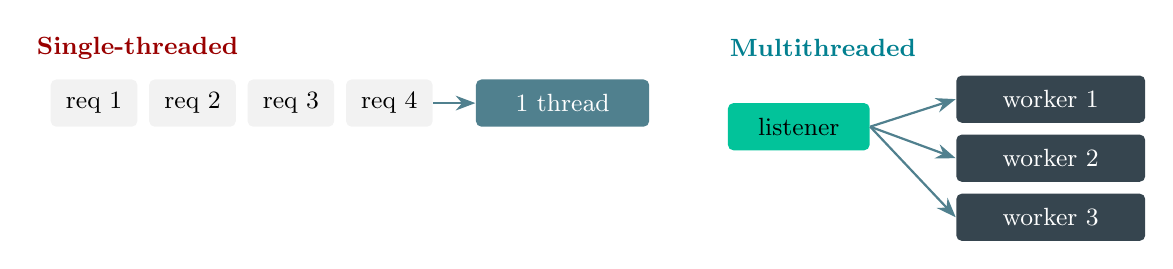
\begin{tikzpicture}[
  b/.style={rectangle,rounded corners=2pt,minimum height=0.6cm,align=center,font=\small},
  arr/.style={-{Stealth[length=2.5mm]},color=slate,thick}]
\node[font=\small\bfseries,text=red!60!black,anchor=west] at (-0.4,1.0) {Single-threaded};
\foreach \i in {1,...,4} \node[b,fill=light,minimum width=1.1cm] (r\i) at (\i*1.25-0.8,0.3) {req \i};
\node[b,fill=slate,text=white,minimum width=2.2cm] (t) at (6.4,0.3) {1 thread};
\draw[arr] (r4) -- (t);
\node[font=\small\bfseries,text=mintdeep,anchor=west] at (8.4,1.0) {Multithreaded};
\node[b,fill=mint,minimum width=1.8cm] (l) at (9.4,0.0) {listener};
\foreach \i in {1,2,3} {
  \node[b,fill=charcoal,text=white,minimum width=2.4cm] (w\i) at (12.6,1.1-\i*0.75) {worker \i};
  \draw[arr] (l.east) -- (w\i.west);
}
\end{tikzpicture}
\caption{A single-threaded server serves requests one by one; a multithreaded server gives each request its own thread.}
\end{figure}

The same idea appears in almost every interactive program. A word processor may have one thread that reads keystrokes, one that redraws the screen, one that checks spelling and one that saves a backup copy every few minutes. A browser loads pages, decodes images and runs scripts in many threads; a game runs rendering, physics, sound and network code in separate threads. In each case the threads work on the \emph{same} data (document, page, game world), so they must share memory.

\subsection{What is a thread?}

\begin{keyidea}[Definition]
A \textbf{thread} is a basic unit of CPU utilisation. It consists of a \emph{thread ID}, a \emph{program counter}, a \emph{register set} and a \emph{stack}. It shares with the other threads of the same process the code section, the data section and the operating-system resources such as open files.
\end{keyidea}

A traditional, ``heavyweight'' process is simply a process with exactly one thread. A multithreaded process has several program counters: several places in the same program are being executed at the same time.

\begin{figure}[H]
\centering
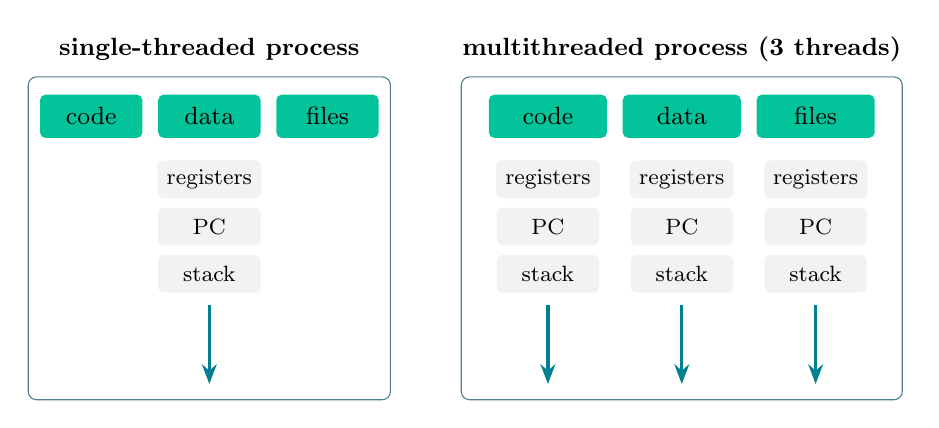
\begin{tikzpicture}[
  sh/.style={rectangle,rounded corners=2pt,fill=mint,minimum width=1.3cm,minimum height=0.55cm,font=\small},
  pr/.style={rectangle,rounded corners=2pt,fill=light,minimum width=1.3cm,minimum height=0.48cm,font=\footnotesize},
  th/.style={-{Stealth[length=2.5mm]},very thick,color=mintdeep}]
% single
\draw[slate,rounded corners=3pt] (-0.2,-3.6) rectangle (4.4,0.5);
\node[font=\small\bfseries] at (2.1,0.85) {single-threaded process};
\foreach \x/\t in {0.6/code,2.1/data,3.6/files} \node[sh] at (\x,0) {\t};
\node[pr] at (2.1,-0.8) {registers}; \node[pr] at (2.1,-1.4) {PC}; \node[pr] at (2.1,-2.0) {stack};
\draw[th] (2.1,-2.4) -- (2.1,-3.4);
% multi
\draw[slate,rounded corners=3pt] (5.3,-3.6) rectangle (10.9,0.5);
\node[font=\small\bfseries] at (8.1,0.85) {multithreaded process (3 threads)};
\foreach \x/\t in {6.4/code,8.1/data,9.8/files} \node[sh,minimum width=1.5cm] at (\x,0) {\t};
\foreach \x in {6.4,8.1,9.8} {
  \node[pr] at (\x,-0.8) {registers}; \node[pr] at (\x,-1.4) {PC}; \node[pr] at (\x,-2.0) {stack};
  \draw[th] (\x,-2.4) -- (\x,-3.4);
}
\end{tikzpicture}
\caption{Mint: shared by all threads of the process. Grey: one private copy per thread. Each arrow is one thread of execution.}
\end{figure}

In terms of Week~3, the PCB is split in two: a per-process part (memory map, open files, user ID) and a small per-thread part (state, saved registers and program counter, stack pointer). Linux calls every thread a \emph{task} and gives it its own kernel record; the threads of one process simply point to the same memory map and the same table of open files. Older texts call threads \term{lightweight processes} (LWP); the abbreviation still appears in the output of \cmd{ps}.

\subsection{What is shared, what is private?}

\begin{center}
\renewcommand{\arraystretch}{1.3}
\begin{tabularx}{\linewidth}{>{\raggedright\arraybackslash}p{4.4cm} l >{\raggedright\arraybackslash}X}
\toprule
\textbf{Item} & \textbf{Threads\dots} & \textbf{Why} \\
\midrule
Code (text section) & share & All threads run functions of the same program. \\
Global data and heap & share & A global variable or a \cmd{malloc}'ed array is visible to every thread. \\
Open files, PID, user ID & share & Resources belong to the process, not to a thread. \\
Program counter and registers & private & Each thread is at its own place in the code. \\
Stack (local variables) & private & Each thread has its own chain of function calls. \\
Thread ID, scheduling state & private & The OS schedules each thread separately. \\
\bottomrule
\end{tabularx}
\end{center}

Sharing is the whole point of threads --- and also their main danger. If two threads update the same variable at the same moment, updates can be lost. This is a \term{race condition}, the central topic of the second half of Week~5.

\subsection{Benefits of multithreading}

\begin{enumerate}[leftmargin=1.4em]
  \item \textbf{Responsiveness.} If one thread blocks (waits for I/O) or performs a long computation, the other threads keep running. The familiar ``application not responding'' message usually means that the single thread handling the user interface is busy with something else.
  \item \textbf{Resource sharing.} Threads share the memory and resources of their process automatically. Separate processes must use explicit mechanisms such as shared memory or pipes to cooperate.
  \item \textbf{Economy.} Creating a thread and switching between threads of the same process are much cheaper than for processes, because no new address space has to be created or switched. We measure this in Section~\ref{sec:createcost}.
  \item \textbf{Scalability.} On a multicore processor, the threads of one process can run in parallel on different cores. A single-threaded process can use only one core, however many the machine has.
\end{enumerate}

\begin{histnote}[Why threads became essential]
Until about 2005, every new generation of processors ran at a higher clock frequency, so old single-threaded programs became faster automatically. Then power consumption and heat stopped the growth of clock speeds at roughly $3$--$5$~GHz. Chip makers used the extra transistors to put several cores on one chip instead. Since then, a program becomes faster on new hardware only if it can use several cores --- that is, only if it is multithreaded (or split into several processes).
\end{histnote}

% =====================================================================
\section{Multicore Programming}

\subsection{Concurrency versus parallelism}

These two words are often confused.

\begin{itemize}
  \item A system is \term{concurrent} if it supports more than one task \emph{making progress}. On a single core, the OS achieves this by switching between threads every few milliseconds; to a human, the threads appear to run simultaneously.
  \item A system is \term{parallel} if it can perform more than one task \emph{at the same instant}. This needs at least two cores.
\end{itemize}

\begin{figure}[H]
\centering
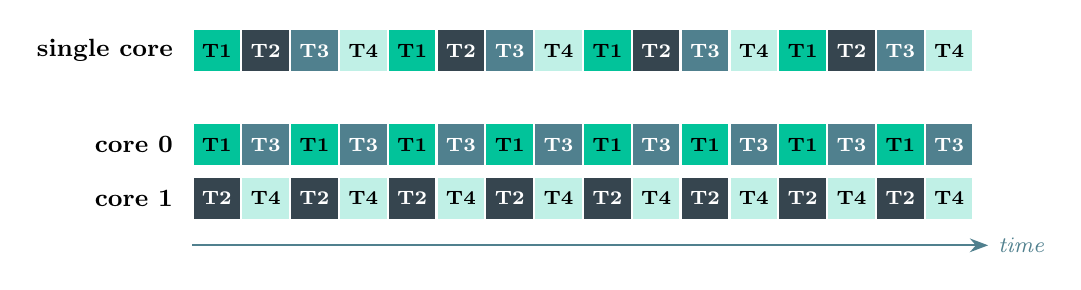
\begin{tikzpicture}[x=0.62cm]
\node[font=\small\bfseries,anchor=east] at (-0.2,1.875) {single core};
\node[font=\small\bfseries,anchor=east] at (-0.2,0.675) {core 0};
\node[font=\small\bfseries,anchor=east] at (-0.2,0.0) {core 1};
\foreach \i in {0,...,15} {
  \pgfmathtruncatemacro{\k}{mod(\i,4)}
  \ifcase\k \def\c{mint}\def\tc{black}\or \def\c{charcoal}\def\tc{white}\or \def\c{slate}\def\tc{white}\or \def\c{mint!25}\def\tc{black}\fi
  \pgfmathtruncatemacro{\tn}{\k+1}
  \fill[\c,draw=white,thick] (\i,1.6) rectangle ++(1,0.55); \node[font=\scriptsize\bfseries,text=\tc] at (\i+0.5,1.875) {T\tn};
  \pgfmathtruncatemacro{\m}{mod(\i,2)}
  \ifcase\m \def\ca{mint}\def\cb{charcoal}\def\ta{black}\def\tb{white}\def\na{1}\def\nb{2}\or \def\ca{slate}\def\cb{mint!25}\def\ta{white}\def\tb{black}\def\na{3}\def\nb{4}\fi
  \fill[\ca,draw=white,thick] (\i,0.4) rectangle ++(1,0.55); \node[font=\scriptsize\bfseries,text=\ta] at (\i+0.5,0.675) {T\na};
  \fill[\cb,draw=white,thick] (\i,-0.275) rectangle ++(1,0.55); \node[font=\scriptsize\bfseries,text=\tb] at (\i+0.5,0.0) {T\nb};
}
\draw[-{Stealth},slate,thick] (0,-0.6) -- (16.3,-0.6) node[right,font=\footnotesize\itshape] {time};
\end{tikzpicture}
\caption{Four threads on one core (concurrency without parallelism) and on two cores (concurrency with parallelism).}
\end{figure}

Parallelism implies concurrency, but not the other way round. The test machine used for this week's measurements has two cores (\cmd{nproc} prints \texttt{2}).

\subsection{Programming challenges}

Writing programs that use several cores well is hard. Five challenges are usually listed:
\begin{enumerate}[leftmargin=1.4em]
  \item \textbf{Identifying tasks:} finding parts of the work that can run independently.
  \item \textbf{Balance:} giving each core a similar amount of work; otherwise some cores sit idle while one finishes.
  \item \textbf{Data splitting:} dividing the data so that each thread works on its own part.
  \item \textbf{Data dependency:} if task~B needs the result of task~A, B must wait for A. The threads must be \emph{synchronised} (Week~5).
  \item \textbf{Testing and debugging:} the threads can interleave in very many different orders; a bug may appear only once in a million runs.
\end{enumerate}

There are two basic kinds of parallelism. In \term{data parallelism} the same operation is applied to different parts of the data; our array-sum program (Section~\ref{sec:arraysum}) is an example. In \term{task parallelism} different threads perform different operations, like the word-processor threads above. Real programs often mix both.

\subsection{Amdahl's law}

Almost every program has a part that cannot be split among cores: reading the input, combining partial results, printing the answer. Gene Amdahl (IBM) observed in 1967 that this \emph{serial} part limits the speedup that any number of cores can deliver.

Let the running time on one core be $1$ (we normalise it), and let $S$ be the fraction of that time that is serial, $0 \le S \le 1$. The remaining fraction $1-S$ can be divided perfectly among $N$ cores. Then
\[
T(1) = S + (1-S) = 1, \qquad T(N) = S + \frac{1-S}{N}.
\]
The \term{speedup} is the ratio of the old time to the new time:
\begin{keyidea}[Amdahl's law]
\[
\text{speedup}(N) = \frac{T(1)}{T(N)} \;\le\; \frac{1}{S + \dfrac{1-S}{N}},
\qquad
\lim_{N\to\infty} \text{speedup}(N) = \frac{1}{S}.
\]
\end{keyidea}
The inequality sign reminds us that this is a best case: real programs also pay for creating threads, synchronising them and sharing memory bandwidth.

\begin{example}[75\,\% parallel, 25\,\% serial]
Take $S = 0.25$, so $1-S = 0.75$.
\begin{align*}
N=2:&\quad \frac{1}{0.25 + 0.75/2} = \frac{1}{0.625} = 1.60,\\
N=4:&\quad \frac{1}{0.25 + 0.75/4} = \frac{1}{0.4375} \approx 2.29,\\
N=8:&\quad \frac{1}{0.25 + 0.75/8} = \frac{1}{0.34375} \approx 2.91,\\
N=16:&\quad \frac{1}{0.25 + 0.75/16} = \frac{1}{0.296875} \approx 3.37,\\
N\to\infty:&\quad \frac{1}{0.25} = 4.
\end{align*}
Doubling the hardware from $8$ to $16$ cores raises the speedup only from $2.91$ to $3.37$. No number of cores can make this program more than $4$ times faster.
\end{example}

\begin{figure}[H]
\centering
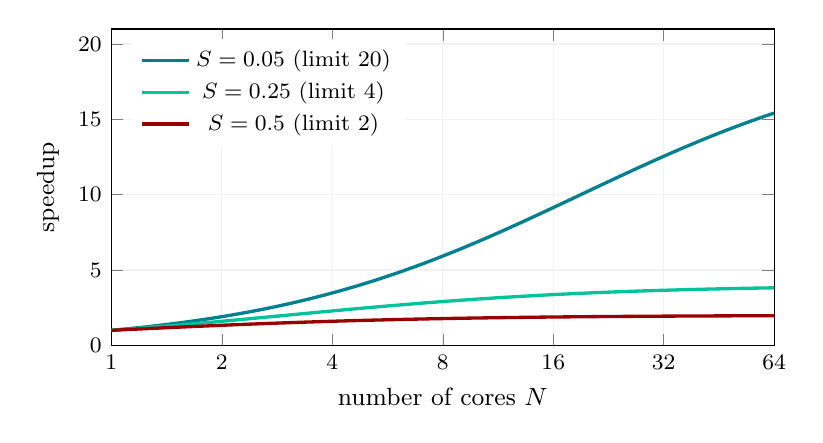
\begin{tikzpicture}
\begin{axis}[width=10cm,height=5.6cm,xmode=log,log basis x=2,xmin=1,xmax=64,ymin=0,ymax=21,
  xlabel={number of cores $N$},ylabel={speedup},xtick={1,2,4,8,16,32,64},xticklabels={1,2,4,8,16,32,64},
  legend pos=north west,legend style={font=\footnotesize,draw=none},grid=major,grid style={light},
  tick label style={font=\footnotesize},label style={font=\small}]
\addplot[mintdeep,very thick,domain=1:64,samples=60] {1/(0.05+0.95/x)};
\addplot[mint,very thick,domain=1:64,samples=60] {1/(0.25+0.75/x)};
\addplot[red!60!black,very thick,domain=1:64,samples=60] {1/(0.5+0.5/x)};
\legend{$S=0.05$ (limit 20),$S=0.25$ (limit 4),$S=0.5$ (limit 2)}
\end{axis}
\end{tikzpicture}
\caption{Amdahl's law: the speedup flattens out at $1/S$.}
\end{figure}

The practical lesson: \emph{first make the serial part small, then add cores.} This is why programs for graphics processors, which have thousands of cores, are designed to keep the serial part tiny.

% =====================================================================
\section{User Threads, Kernel Threads and Multithreading Models}

\subsection{User-level and kernel-level threads}

Threads can be provided at two levels.

\paragraph{User-level threads} are managed by a library inside the process. The kernel knows nothing about them: it sees one ordinary single-threaded process.
\begin{itemize}
  \item[\textcolor{mintdeep}{$+$}] Creating and switching threads are ordinary function calls: very fast, no system call.
  \item[\textcolor{red!60!black}{$-$}] If one thread makes a blocking system call (e.g.\ \cmd{read()} from a slow device), the kernel blocks the whole process, and all its threads stop.
  \item[\textcolor{red!60!black}{$-$}] The kernel schedules only one entity, so the threads cannot run on two cores at once.
\end{itemize}

\paragraph{Kernel-level threads} are created, scheduled and managed by the operating-system kernel; each has its own kernel record.
\begin{itemize}
  \item[\textcolor{mintdeep}{$+$}] If one thread blocks, the kernel runs another thread of the same process.
  \item[\textcolor{mintdeep}{$+$}] The threads of one process can run in parallel on several cores.
  \item[\textcolor{red!60!black}{$-$}] Creating and switching threads need system calls and are slower than for user threads.
\end{itemize}

Every user thread must eventually run on some kernel thread. The way user threads are mapped onto kernel threads is called the \term{multithreading model}.

\subsection{The three models}

\begin{figure}[H]
\centering
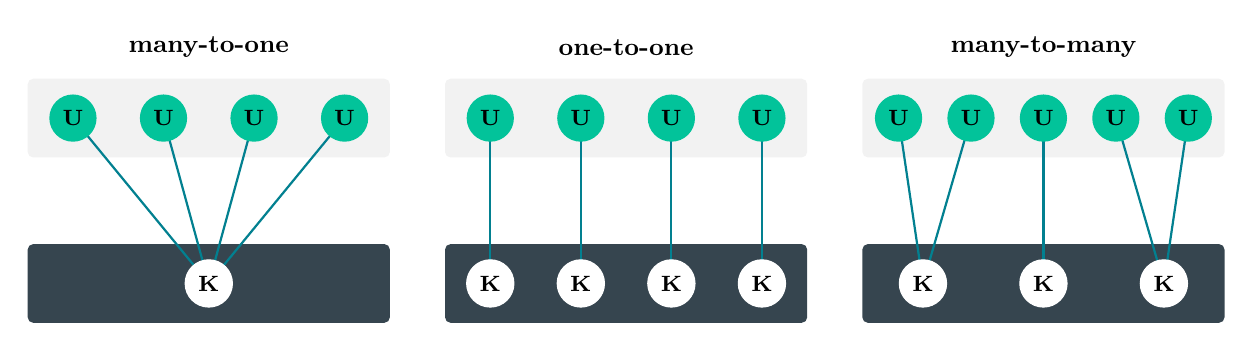
\begin{tikzpicture}[
  u/.style={circle,fill=mint,minimum size=0.6cm,inner sep=0pt,font=\footnotesize\bfseries},
  k/.style={circle,fill=white,draw=white,minimum size=0.6cm,inner sep=0pt,font=\footnotesize\bfseries},
  l/.style={mintdeep,thick}]
\foreach \ox/\title in {0/{many-to-one},5.3/{one-to-one},10.6/{many-to-many}} {
  \fill[light,rounded corners=2pt] (\ox,1.6) rectangle ++(4.6,1.0);
  \fill[charcoal,rounded corners=2pt] (\ox,-0.5) rectangle ++(4.6,1.0);
  \node[font=\small\bfseries] at (\ox+2.3,3.0) {\title};
}
% many-to-one
\foreach \i in {0,...,3} { \draw[l] (0.575+\i*1.15,2.1) -- (2.3,0); }
\foreach \i in {0,...,3} \node[u] at (0.575+\i*1.15,2.1) {U};
\node[k] at (2.3,0) {K};
% one-to-one
\foreach \i in {0,...,3} { \draw[l] (5.875+\i*1.15,2.1) -- (5.875+\i*1.15,0); \node[u] at (5.875+\i*1.15,2.1) {U}; \node[k] at (5.875+\i*1.15,0) {K}; }
% many-to-many
\foreach \a/\b in {0/0,1/0,2/1,3/2,4/2} \draw[l] (11.06+\a*0.92,2.1) -- (11.37+\b*1.53,0);
\foreach \a in {0,...,4} \node[u] at (11.06+\a*0.92,2.1) {U};
\foreach \b in {0,1,2} \node[k] at (11.37+\b*1.53,0) {K};
\end{tikzpicture}
\caption{The three multithreading models. Light band: user space with user threads (U); dark band: kernel space with kernel threads (K).}
\end{figure}

\paragraph{Many-to-one.} Many user threads are mapped onto a single kernel thread; thread management is done by a library in user space. It is fast, but one blocking system call blocks every thread, and only one thread can be in the kernel at a time, so the model cannot use multiple cores. Examples: Solaris Green Threads, GNU Portable Threads. Few systems use it today.

\paragraph{One-to-one.} Each user thread is mapped onto its own kernel thread. A blocking call blocks only the calling thread, and threads run in parallel on multicore processors. The cost is that every user thread needs a kernel thread, so creating a thread requires a system call and very large numbers of threads burden the kernel. \textbf{Linux and Windows use the one-to-one model.} On Linux, \cmd{pthread\_create()} calls the \cmd{clone()} system call, and every thread gets its own thread ID (TID) in the kernel.

\paragraph{Many-to-many.} Many user threads are multiplexed onto a smaller or equal number of kernel threads. The program can create as many user threads as it likes, and they can still run in parallel; a blocking call does not stop everything. The price is complexity: a scheduler in the library and the scheduler in the kernel must cooperate. A common variation, the \emph{two-level model}, also allows a user thread to be bound to its own kernel thread. Operating-system kernels abandoned this model for one-to-one, but language runtimes revived it: Go's \emph{goroutines} and Java's \emph{virtual threads} (Java~21, 2023) run millions of lightweight tasks on a few kernel threads.

\begin{center}
\renewcommand{\arraystretch}{1.3}
\begin{tabular}{@{}lllll@{}}
\toprule
\textbf{Model} & \textbf{User : kernel} & \textbf{Parallel?} & \textbf{Blocking call stops\dots} & \textbf{Used by} \\
\midrule
Many-to-one & $N:1$ & no & all threads & Green threads (old) \\
One-to-one & $1:1$ & yes & only that thread & Linux, Windows \\
Many-to-many & $N:M$, $M\le N$ & yes & only that thread & Go, Java virtual threads \\
\bottomrule
\end{tabular}
\end{center}


% =====================================================================
\section{Thread Libraries and Hands-on Pthreads}
\label{sec:handson}

A \term{thread library} gives the programmer an API for creating and managing threads. The three main libraries are \textbf{POSIX Pthreads} (Linux, macOS and other UNIX systems), the \textbf{Windows thread API}, and \textbf{Java threads}. On Linux and Windows, Java threads are mapped one-to-one onto kernel threads by the Java virtual machine.

Pthreads is a \emph{specification} (part of the POSIX standard), not an implementation. On Linux it is implemented in the C library (glibc, under the name NPTL) on top of the \cmd{clone()} system call. The essential calls are:

\begin{center}
\renewcommand{\arraystretch}{1.3}
\begin{tabularx}{\linewidth}{>{\ttfamily}l X}
\toprule
\textrm{\textbf{Call}} & \textbf{What it does} \\
\midrule
pthread\_create(\&t, NULL, f, arg) & Start a new thread that runs \cmd{f(arg)}; its handle is stored in \cmd{t}. \\
pthread\_join(t, \&result) & Wait until thread \cmd{t} has finished (like \cmd{wait()} for processes). \\
pthread\_exit(value) & End the calling thread (returning from \cmd{f} does the same). \\
pthread\_self() & Return the calling thread's own handle. \\
gcc -pthread prog.c & Compile and link with the Pthreads library. \\
\bottomrule
\end{tabularx}
\end{center}

A thread function always has the form \cmd{void *f(void *arg)}: it receives one generic pointer and returns one. To pass several values, pass a pointer to a \cmd{struct}.

The programs below are in the \texttt{code/} folder next to these notes, with a \texttt{Makefile} (type \cmd{make}). They were compiled with \cmd{gcc -Wall -O2 -pthread} and run on a Linux virtual machine with two cores that was shared with other jobs. As in Week~2, you are not expected to write C in this course: read the comments and focus on what the program does.

\subsection{Example 1: is a thread really cheaper than a process?}
\label{sec:createcost}

\lstinputlisting[caption={}]{../code/create_cost_excerpt.c}

\begin{lstlisting}[style=term]
$ ./create_cost
fork + wait          :  205.5 us per process
pthread_create + join:   51.9 us per thread
a thread is about 4 times cheaper to create
\end{lstlisting}

(\texttt{us} means microseconds, $\mu$s.) \cmd{fork()} must create a new address space: copy the page tables and many kernel structures, even though the memory pages themselves are shared copy-on-write until someone writes to them. A new thread needs only a stack and a small kernel record. On a fast physical machine thread creation often takes only $10$--$20\ \mu$s and the ratio is larger; textbooks quote factors of $10$ to $30$. Our ratio of about $4$ comes from a virtual machine, where some operations are slower.

\subsection{Example 2: hello from three threads}

\lstinputlisting[caption={}]{../code/thread_hello.c}

\begin{lstlisting}[style=term]
$ gcc -Wall -O2 -pthread thread_hello.c -o thread_hello
$ ./thread_hello
main    : PID = 6351, TID = 6351
thread 1: PID = 6351, TID = 6352
thread 3: PID = 6351, TID = 6354
thread 2: PID = 6351, TID = 6353
main    : all threads done, shared_counter = 3
\end{lstlisting}

Three observations:
\begin{itemize}
  \item All threads print the \emph{same} PID: they belong to one process. Each has its \emph{own} TID, because each is a separate kernel thread (one-to-one model). The main thread's TID equals the PID.
  \item Thread~3 printed before thread~2. The order is decided by the scheduler and changes from run to run; a program must never rely on it.
  \item \cmd{shared\_counter} ends at $3$: the global variable is shared. But \cmd{shared\_counter++} is not safe when threads run at the same time (it is really ``load, add, store''). With three increments the bug almost never shows; with millions it does. We fix this in Week~5.
\end{itemize}

\paragraph{Seeing the threads.} Each worker sleeps for two seconds, which gives us time to look at the running process. The option \cmd{-L} of \cmd{ps} prints one line per thread (some columns removed):

\begin{lstlisting}[style=term]
$ ./thread_hello &
$ ps -eLf | grep thread_hello
UID    PID  PPID   LWP  C NLWP CMD
root 27241 27234 27241  0    4 ./thread_hello
root 27241 27234 27243  0    4 ./thread_hello
root 27241 27234 27244  0    4 ./thread_hello
root 27241 27234 27245  0    4 ./thread_hello
$ ls /proc/27241/task
27241  27243  27244  27245
$ grep Threads /proc/27241/status
Threads:   4
\end{lstlisting}

The PID is the same on every line; \texttt{LWP} (lightweight process) is the thread ID and \texttt{NLWP} the number of threads: the main thread plus three workers. The directory \cmd{/proc/<pid>/task/} contains one subdirectory per thread. Other tools: \cmd{top -H} or \cmd{htop} show threads interactively; on Windows, Task Manager $\to$ \emph{Details} can show a \emph{Threads} column.

\subsection{Example 3: summing an array with $T$ threads}
\label{sec:arraysum}

\lstinputlisting[caption={}]{../code/array_sum_excerpt.c}

The array of $N = 10^{8}$ integers ($400$ MB) is cut into $T$ equal slices. Thread $k$ sums the elements with indices from $kN/T$ up to (but not including) $(k+1)N/T$ into its own slot \cmd{partial[k]}. Because no two threads write to the same variable, no locks are needed. The main thread waits for every thread with \cmd{pthread\_join()} and adds the partial sums. The full program \texttt{code/array\_sum.c} also measures the time with \cmd{clock\_gettime()} and sums the array $20$ times, so that the measured time is long enough to be stable; the correct result is $10^{7} \times (0+1+\dots+9) \times 20 = 10^{7}\times 45\times 20 = 9\times10^{9}$, which every run reproduced.

\begin{lstlisting}[style=term]
$ nproc
2
$ ./array_sum 1
threads = 1   sum = 9000000000   time = 1.686 s
$ ./array_sum 2
threads = 2   sum = 9000000000   time = 0.999 s
$ ./array_sum 4
threads = 4   sum = 9000000000   time = 0.855 s
\end{lstlisting}

Because the machine was shared with other jobs, single runs varied by up to about $\pm 30\%$. We therefore ran each case $9$ times and report the median:

\begin{center}
\renewcommand{\arraystretch}{1.3}
\begin{tabular}{@{}cccc@{}}
\toprule
\textbf{Threads $T$} & \textbf{Median time} & \textbf{Best time} & \textbf{Speedup (median)} \\
\midrule
1 & $1.564$ s & $1.498$ s & $1.00$ \\
2 & $0.932$ s & $0.761$ s & $1.564/0.932 \approx 1.68$ \\
4 & $0.855$ s & $0.728$ s & $1.564/0.855 \approx 1.83$ \\
\bottomrule
\end{tabular}
\end{center}

\paragraph{Interpretation.} Two threads give a speedup of $1.68$, good but below the ideal value $2$. Four threads are hardly better, because the machine has only two cores: at any instant at most two threads can run. (On a busy machine four threads can be slightly faster than two simply because the process then receives a larger share of the CPU time, but never faster than the number of cores allows.) If we pretend that Amdahl's law describes the measurement, we can solve for $S$:
\[
1.68 = \frac{1}{S + (1-S)/2} \;\Longrightarrow\; S + \frac{1-S}{2} = \frac{1}{1.68} \;\Longrightarrow\; S = \frac{2}{1.68} - 1 \approx 0.19 .
\]
Here the ``serial part'' is not really code that cannot be split: it is the time to create and join threads, the competition of both cores for the same memory bandwidth (summing integers is limited by memory speed, not arithmetic), and the other jobs on the machine. Amdahl's law is a model and an upper bound, not an exact prediction.


% =====================================================================
\section{CPU Scheduling: Basic Concepts}

On a machine with one core, only one thread can run at a time; with $N$ cores, at most $N$. All other runnable threads must wait. Whenever a core becomes free, the operating system must choose which thread runs next. This choice is \term{CPU scheduling}. Textbooks speak of ``process scheduling''; on Linux and Windows the kernel actually schedules kernel threads, but everything below applies to both, and we follow the textbook in saying ``process''.

\subsection{The CPU--I/O burst cycle}

Process execution consists of a \emph{cycle} of CPU execution and I/O waiting. A process runs for a while (a \term{CPU burst}), then waits for I/O (an \term{I/O burst}), then runs again, and so on, until a final CPU burst ends with a request to terminate.

\begin{figure}[H]
\centering
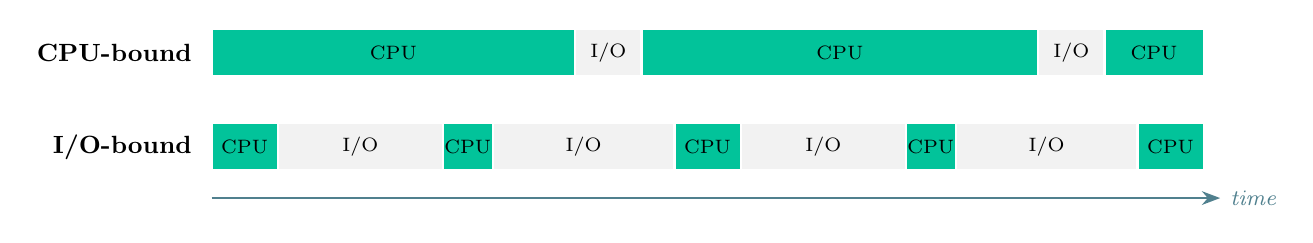
\begin{tikzpicture}[x=0.42cm]
\node[font=\small\bfseries,anchor=east] at (-0.3,1.6) {CPU-bound};
\node[font=\small\bfseries,anchor=east] at (-0.3,0.4) {I/O-bound};
\foreach \a/\b/\c/\t in {0/11/mint/CPU,11/13/light/{I/O},13/25/mint/CPU,25/27/light/{I/O},27/30/mint/CPU} {
  \fill[\c,draw=white,thick] (\a,1.3) rectangle (\b,1.9);
  \node[font=\scriptsize] at ({(\a+\b)/2},1.6) {\t};
}
\foreach \a/\b/\c/\t in {0/2/mint/CPU,2/7/light/{I/O},7/8.5/mint/CPU,8.5/14/light/{I/O},14/16/mint/CPU,16/21/light/{I/O},21/22.5/mint/CPU,22.5/28/light/{I/O},28/30/mint/CPU} {
  \fill[\c,draw=white,thick] (\a,0.1) rectangle (\b,0.7);
  \node[font=\scriptsize] at ({(\a+\b)/2},0.4) {\t};
}
\draw[-{Stealth},slate,thick] (0,-0.25) -- (30.5,-0.25) node[right,font=\footnotesize\itshape] {time};
\end{tikzpicture}
\caption{A CPU-bound process has few, long CPU bursts; an I/O-bound process has many short ones.}
\end{figure}

\begin{itemize}
  \item A \term{CPU-bound} process spends most of its time computing: video encoding, compiling, scientific simulation.
  \item An \term{I/O-bound} process spends most of its time waiting for I/O and has many short CPU bursts: a text editor, a web server, a file copy.
\end{itemize}

Measurements of real systems show that the lengths of CPU bursts follow a typical pattern: a large number of short bursts (a few milliseconds) and a small number of long ones. The distribution is roughly exponential. Scheduling algorithms are designed around this fact (Week~5). While a process waits for I/O, the CPU would be idle --- unless the scheduler gives it to another process: the idea of multiprogramming from Week~1.

\subsection{Example 4: CPU-bound versus I/O-bound, measured}

\lstinputlisting[caption={}]{../code/burst_excerpt.c}

The shell command \cmd{time} reports three numbers: \texttt{real} is the elapsed wall-clock time; \texttt{user} and \texttt{sys} are the CPU time the process consumed in user mode and in kernel mode.

\begin{lstlisting}[style=term]
$ time ./burst cpu
cpu: harmonic sum = 20.384191
real    0m1.266s
user    0m1.197s
sys     0m0.001s
$ time ./burst io
io: wrote 1000 blocks of 4 KB, each followed by fsync
real    0m0.384s
user    0m0.000s
sys     0m0.104s
\end{lstlisting}

\begin{example}[How much of the time was the process waiting?]
For the CPU-bound run, $\text{user}+\text{sys} = 1.198$ s $\approx$ real $= 1.266$ s: the process used the CPU almost all the time. For the I/O-bound run,
\[
\frac{\text{user} + \text{sys}}{\text{real}} = \frac{0.000 + 0.104}{0.384} \approx 0.27,
\]
so the process used the CPU only $27\%$ of the time; about $73\%$ of the time it was blocked in \cmd{fsync()}, waiting for the disk. During that time the CPU was free for other processes. Note also that almost all of its CPU time is \texttt{sys}: \cmd{write()} and \cmd{fsync()} are system calls. (The harmonic sum checks out: $\sum_{i=1}^{n} 1/i \approx \ln n + 0.5772$, and $\ln(4\times10^{8}) + 0.5772 \approx 20.384$.)
\end{example}

\subsection{The CPU scheduler and the ready queue}

Whenever the CPU becomes idle, the operating system selects one of the processes in the \term{ready queue} to run. The part of the OS that makes this choice is the \term{short-term scheduler} or \term{CPU scheduler}.

\begin{figure}[H]
\centering
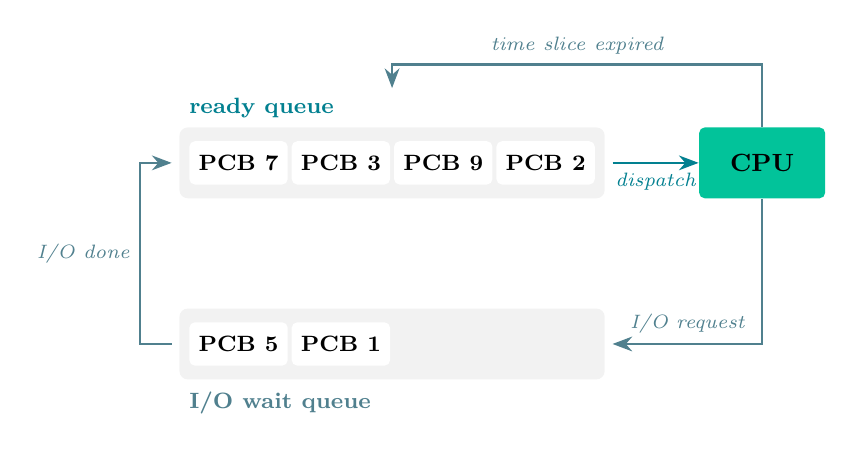
\begin{tikzpicture}[
  pcb/.style={rectangle,rounded corners=2pt,fill=white,minimum width=1.1cm,minimum height=0.55cm,font=\footnotesize\bfseries},
  arr/.style={-{Stealth[length=2.5mm]},color=slate,thick}]
\fill[light,rounded corners=3pt] (0,0) rectangle (5.4,0.9);
\foreach \i/\t in {0/7,1/3,2/9,3/2} \node[pcb] at (0.75+\i*1.3,0.45) {PCB \t};
\node[font=\footnotesize\bfseries,text=mintdeep,anchor=west] at (0,1.15) {ready queue};
\node[rectangle,rounded corners=2pt,fill=mint,minimum width=1.6cm,minimum height=0.9cm,font=\small\bfseries] (cpu) at (7.4,0.45) {CPU};
\draw[arr,mintdeep] (5.5,0.45) -- node[below,font=\scriptsize\itshape]{dispatch} (cpu.west);
\fill[light,rounded corners=3pt] (0,-2.3) rectangle (5.4,-1.4);
\foreach \i/\t in {0/5,1/1} \node[pcb] at (0.75+\i*1.3,-1.85) {PCB \t};
\node[font=\footnotesize\bfseries,text=slate,anchor=west] at (0,-2.6) {I/O wait queue};
\draw[arr] (cpu.south) |- node[pos=0.75,above,font=\scriptsize\itshape]{I/O request} (5.5,-1.85);
\draw[arr] (-0.1,-1.85) -- (-0.5,-1.85) |- node[pos=0.25,left,font=\scriptsize\itshape]{I/O done} (-0.1,0.45);
\draw[arr] (cpu.north) |- node[pos=0.75,above,font=\scriptsize\itshape]{time slice expired} (2.7,1.7) -- (2.7,1.4);
\end{tikzpicture}
\caption{Processes move between the ready queue, the CPU and device wait queues.}
\end{figure}

\begin{itemize}
  \item The ready queue holds the PCBs of exactly those processes that are in the \emph{ready} state of the Week~3 diagram: they could run right now.
  \item The ready queue is not necessarily first-in, first-out. It may be a priority queue, a tree or an unordered list; the order in which processes are taken from it is the \term{scheduling algorithm} (Week~5). Linux keeps its ready tasks in a balanced binary tree (a red--black tree).
  \item The short-term scheduler runs very often --- every few milliseconds --- so it must be fast.
\end{itemize}

\subsection{When does the scheduler have to decide?}

Scheduling decisions may take place in four situations, all visible in the process-state diagram:

\begin{figure}[H]
\centering
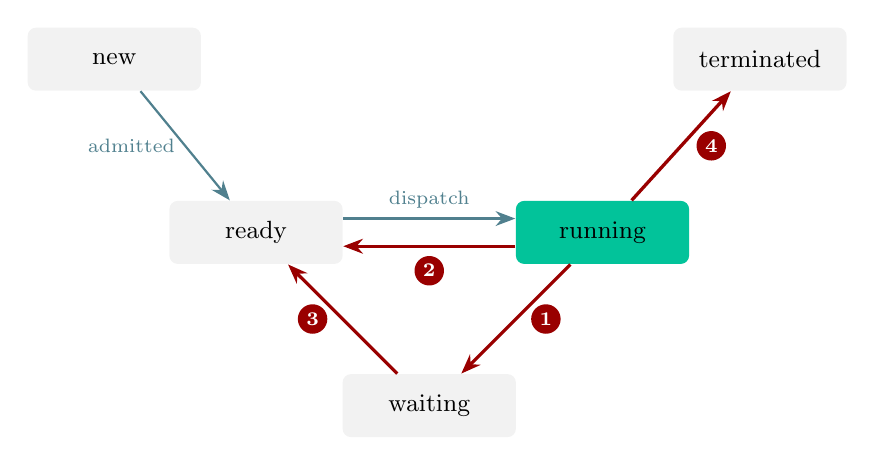
\begin{tikzpicture}[
  st/.style={rectangle,rounded corners=3pt,minimum width=2.2cm,minimum height=0.8cm,font=\small,fill=light},
  arr/.style={-{Stealth[length=2.5mm]},thick,color=slate},
  red/.style={-{Stealth[length=2.5mm]},very thick,color=red!60!black},
  n/.style={circle,fill=red!60!black,text=white,font=\scriptsize\bfseries,inner sep=1.5pt}]
\node[st] (new) at (0,2.2) {new};
\node[st] (ready) at (1.8,0) {ready};
\node[st,fill=mint] (run) at (6.2,0) {running};
\node[st] (wait) at (4.0,-2.2) {waiting};
\node[st] (term) at (8.2,2.2) {terminated};
\draw[arr] (new) -- node[left,font=\scriptsize]{admitted} (ready);
\draw[arr] ([yshift=5pt]ready.east) -- node[above,font=\scriptsize]{dispatch} ([yshift=5pt]run.west);
\draw[red] ([yshift=-5pt]run.west) -- node[below]{\tikz\node[n]{2};} ([yshift=-5pt]ready.east);
\draw[red] (run) -- node[right=2pt]{\tikz\node[n]{1};} (wait);
\draw[red] (wait) -- node[left=2pt]{\tikz\node[n]{3};} (ready);
\draw[red] (run) -- node[right=2pt]{\tikz\node[n]{4};} (term);
\end{tikzpicture}
\caption{The four transitions at which a scheduling decision can be made.}
\end{figure}

\begin{enumerate}[leftmargin=1.4em]
  \item A process switches from \emph{running} to \emph{waiting}: it requests I/O or calls \cmd{wait()} for a child.
  \item A process switches from \emph{running} to \emph{ready}: an interrupt occurs, for example the timer signals that its time slice is over.
  \item A process switches from \emph{waiting} to \emph{ready}: its I/O has completed.
  \item A process \emph{terminates}.
\end{enumerate}

In situations~1 and~4 there is no choice: the CPU has become free, and a new process \emph{must} be selected (if the ready queue is not empty). In situations~2 and~3 there is a choice: the OS \emph{may} let the current process continue or switch to another one --- for example to a more important process that has just become ready.

\subsection{Non-preemptive and preemptive scheduling}

\begin{itemize}
  \item Under \term{non-preemptive} (or \emph{cooperative}) scheduling, the scheduler runs only in situations~1 and~4. Once a process has the CPU, it keeps it until it blocks or terminates. This is simple, but one long or misbehaving process can make all others wait. Windows~3.x and the classic Mac~OS (before OS~X) worked this way: a program stuck in an infinite loop froze the whole computer.
  \item Under \term{preemptive} scheduling, the scheduler can also run in situations~2 and~3: the OS can take the CPU away from a running process, using the timer interrupt. All modern general-purpose operating systems --- Windows, macOS, Linux, Android, iOS --- are preemptive.
\end{itemize}

Preemption gives better responsiveness and protects the system from runaway programs, but it has a price: a process can be interrupted at \emph{any} instruction, even in the middle of updating data shared with another process or thread. This is how race conditions arise, and why Week~5 continues with synchronisation.

\subsection{The dispatcher}

The scheduler decides \emph{which} process runs next; the \term{dispatcher} is the module that actually gives it the CPU. Its three jobs are:
\begin{enumerate}[leftmargin=1.4em]
  \item switch context: save the state of the old process into its PCB and load the state of the new one;
  \item switch to user mode;
  \item jump to the proper location in the new program (its saved program counter).
\end{enumerate}

The time the dispatcher needs to stop one process and start another is the \term{dispatch latency}. It is pure overhead: no useful work is done during it.

\begin{figure}[H]
\centering
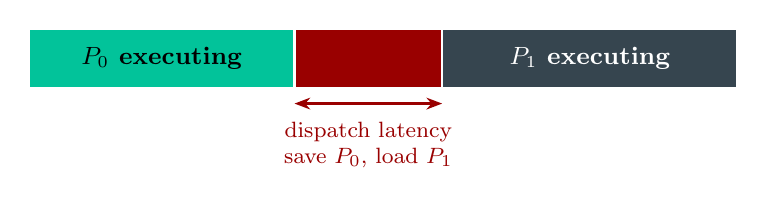
\begin{tikzpicture}[x=0.75cm]
\fill[mint,draw=white,thick] (0,0) rectangle (4.5,0.75); \node[font=\small\bfseries] at (2.25,0.375) {$P_0$ executing};
\fill[red!60!black,draw=white,thick] (4.5,0) rectangle (7,0.75);
\fill[charcoal,draw=white,thick] (7,0) rectangle (12,0.75); \node[font=\small\bfseries,text=white] at (9.5,0.375) {$P_1$ executing};
\draw[{Stealth[length=2mm]}-{Stealth[length=2mm]},thick,red!60!black] (4.5,-0.2) -- (7,-0.2) node[midway,below=3pt,font=\footnotesize,align=center,text=red!60!black] {dispatch latency\\save $P_0$, load $P_1$};
\end{tikzpicture}
\caption{Dispatch latency (not to scale: it is microseconds, a time slice is milliseconds).}
\end{figure}

Dispatch latency is small, typically a few microseconds, but it happens very often. The command \cmd{vmstat 1} prints, among other things, the number of context switches per second in the column \texttt{cs}. On our otherwise idle test machine two consecutive one-second samples showed $487$ and $614$; a busy server easily reaches tens of thousands.

\paragraph{Voluntary and involuntary context switches.} Linux counts separately how often a process gave up the CPU itself, because it blocked (a \emph{voluntary} switch, situation~1), and how often the scheduler took the CPU away (an \emph{involuntary} switch, situation~2). The GNU \cmd{time} program with option \cmd{-v} reports both (other lines, including the user and system times, removed):

\begin{lstlisting}[style=term]
$ /usr/bin/time -v ./burst cpu
  Elapsed (wall clock) time (h:mm:ss or m:ss): 0:01.22
  Voluntary context switches: 1
  Involuntary context switches: 50
$ /usr/bin/time -v ./burst io
  Elapsed (wall clock) time (h:mm:ss or m:ss): 0:00.46
  Voluntary context switches: 3714
  Involuntary context switches: 0
\end{lstlisting}

The CPU-bound program almost never blocked, but it was preempted $50$ times in $1.22$~s, on average about once every $24$~ms. The I/O-bound program was never preempted but blocked $3714$ times (each \cmd{fsync()} may wait more than once, e.g.\ for the file-system journal). The same counters are visible for a running process in \cmd{/proc/<pid>/status} (fields \nolinkurl{voluntary_ctxt_switches} and \nolinkurl{nonvoluntary_ctxt_switches}).

% =====================================================================
\section{Scheduling Criteria}

Different scheduling algorithms favour different processes. To compare them we need measurable criteria.

\begin{center}
\renewcommand{\arraystretch}{1.3}
\begin{tabularx}{\linewidth}{>{\raggedright\arraybackslash}p{3.0cm} X l}
\toprule
\textbf{Criterion} & \textbf{Definition} & \textbf{Goal} \\
\midrule
CPU utilisation & Fraction of time the CPU is busy with useful work; on a real system from about $40\%$ (light load) to $90\%$ (heavy load). & maximise \\
Throughput & Number of processes completed per unit of time. & maximise \\
Turnaround time & Time from the arrival (submission) of a process to its completion, including waiting in the ready queue, executing and doing I/O. & minimise \\
Waiting time & Total time a process spends waiting in the \emph{ready queue}. & minimise \\
Response time & Time from arrival until the process first gets the CPU (its first response). & minimise \\
\bottomrule
\end{tabularx}
\end{center}

The scheduling algorithm does not change how long a process computes or how long its I/O takes; it only changes how long the process sits in the ready queue. That is why \emph{waiting time} is the criterion most directly affected by the scheduler.

\subsection{The definitions as formulas}

For a process with arrival time $T_{\text{arrival}}$, total CPU burst time $T_{\text{burst}}$, first time on the CPU $T_{\text{first run}}$ and completion time $T_{\text{completion}}$, and doing no I/O:
\begin{align*}
T_{\text{turnaround}} &= T_{\text{completion}} - T_{\text{arrival}},\\
T_{\text{waiting}} &= T_{\text{turnaround}} - T_{\text{burst}},\\
T_{\text{response}} &= T_{\text{first run}} - T_{\text{arrival}}.
\end{align*}
If the process also performs I/O, the time spent in I/O must be subtracted as well: $T_{\text{waiting}} = T_{\text{turnaround}} - T_{\text{burst}} - T_{\text{I/O}}$, because waiting time counts only the time in the ready queue. For a set of $n$ processes completed in a time interval of length $T$ during which the CPU was busy for $B$,
\[
\text{CPU utilisation} = \frac{B}{T}, \qquad \text{throughput} = \frac{n}{T}.
\]

\begin{figure}[H]
\centering
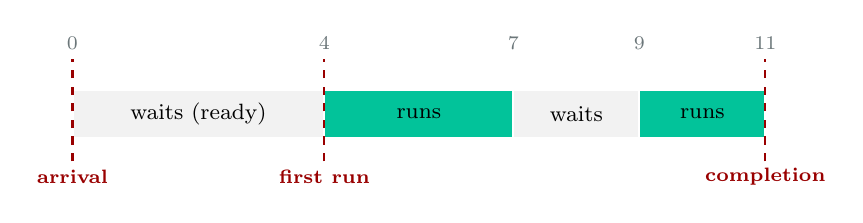
\begin{tikzpicture}[x=0.8cm]
\fill[light,draw=white,thick] (0,0) rectangle (4,0.6); \node[font=\footnotesize] at (2,0.3) {waits (ready)};
\fill[mint,draw=white,thick] (4,0) rectangle (7,0.6); \node[font=\footnotesize] at (5.5,0.3) {runs};
\fill[light,draw=white,thick] (7,0) rectangle (9,0.6); \node[font=\footnotesize] at (8,0.3) {waits};
\fill[mint,draw=white,thick] (9,0) rectangle (11,0.6); \node[font=\footnotesize] at (10,0.3) {runs};
\foreach \t/\l in {0/arrival,4/first run,11/completion} {
  \draw[red!60!black,dashed,thick] (\t,-0.3) -- (\t,1.0);
  \node[font=\scriptsize\bfseries,text=red!60!black] at (\t,-0.5) {\l};
}
\foreach \t in {0,4,7,9,11} \node[font=\scriptsize,text=muted] at (\t,1.2) {$\t$};
\end{tikzpicture}
\caption{A process that is preempted once: burst $=3+2=5$, waiting $=4+2=6$, turnaround $=11$, response $=4$.}
\end{figure}

\begin{example}[Checking the formulas on the picture]
$T_{\text{turnaround}} = 11 - 0 = 11$; $T_{\text{waiting}} = 11 - 5 = 6$, which is indeed $4 + 2$ units in the ready queue; $T_{\text{response}} = 4 - 0 = 4$. For a process like this, response $\le$ waiting $\le$ turnaround. Under non-preemptive scheduling a process waits only once, before its single run, so its response time equals its waiting time.
\end{example}

\subsection{Worked example: four processes in arrival order}

Four processes arrive at a single CPU. We run them in the ``obvious'' order, first come, first served (FCFS), without preemption. Whether this is a good order is the question of Week~5; here we only practise the definitions. All times are in milliseconds.

\begin{center}
\renewcommand{\arraystretch}{1.2}
\begin{tabular}{@{}ccc@{}}
\toprule
\textbf{Process} & \textbf{Arrival} & \textbf{Burst} \\
\midrule
$P_1$ & $0$ & $5$ \\
$P_2$ & $1$ & $3$ \\
$P_3$ & $2$ & $6$ \\
$P_4$ & $16$ & $2$ \\
\bottomrule
\end{tabular}
\end{center}

\textbf{Building the Gantt chart.} At $t=0$ only $P_1$ is present and runs. $P_2$ ($t=1$) and $P_3$ ($t=2$) arrive while $P_1$ runs and wait in the ready queue. At $t=5$, $P_1$ finishes and $P_2$, which arrived first, runs until $t=8$; then $P_3$ runs until $t=14$. Now the ready queue is empty, so the CPU is idle until $P_4$ arrives at $t=16$; $P_4$ runs until $t=18$.

\begin{figure}[H]
\centering
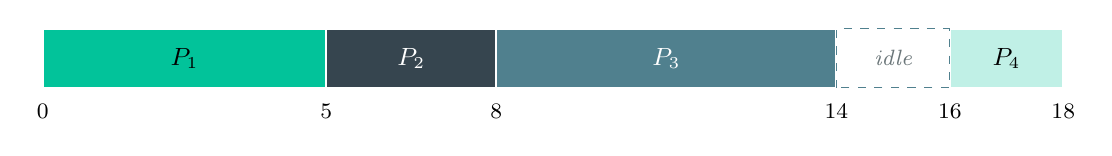
\begin{tikzpicture}[x=0.72cm]
\foreach \a/\b/\l/\c/\tc in {0/5/P_1/mint/black,5/8/P_2/charcoal/white,8/14/P_3/slate/white,16/18/P_4/mint!25/black} {
  \fill[\c,draw=white,thick] (\a,0) rectangle (\b,0.75);
  \node[font=\small\bfseries,text=\tc] at ({(\a+\b)/2},0.375) {$\l$};
}
\draw[slate,dashed] (14,0) rectangle (16,0.75); \node[font=\footnotesize\itshape,text=muted] at (15,0.375) {idle};
\foreach \t in {0,5,8,14,16,18} \node[font=\footnotesize] at (\t,-0.3) {$\t$};
\end{tikzpicture}
\caption{Gantt chart of the worked example (FCFS order).}
\end{figure}

\begin{center}
\renewcommand{\arraystretch}{1.3}
\begin{tabular}{@{}ccccccc@{}}
\toprule
\textbf{Process} & \textbf{Arrival} & \textbf{Burst} & \textbf{Completion} & \textbf{Turnaround} & \textbf{Waiting} & \textbf{Response} \\
\midrule
$P_1$ & $0$ & $5$ & $5$ & $5-0=5$ & $5-5=0$ & $0$ \\
$P_2$ & $1$ & $3$ & $8$ & $8-1=7$ & $7-3=4$ & $4$ \\
$P_3$ & $2$ & $6$ & $14$ & $14-2=12$ & $12-6=6$ & $6$ \\
$P_4$ & $16$ & $2$ & $18$ & $18-16=2$ & $2-2=0$ & $0$ \\
\midrule
\textbf{Average} & & & & $26/4 = 6.5$ & $10/4 = 2.5$ & $2.5$ \\
\bottomrule
\end{tabular}
\end{center}

\begin{itemize}
  \item Average turnaround time $= (5+7+12+2)/4 = 6.5$ ms; average waiting time $= (0+4+6+0)/4 = 2.5$ ms; average response time $= 2.5$ ms (equal to the waiting time, because the scheduling is non-preemptive).
  \item CPU utilisation $= 16\ \text{ms busy} / 18\ \text{ms} \approx 88.9\%$. The idle gap lowers utilisation but does not increase anybody's waiting time.
  \item Throughput $= 4 / 18\ \text{ms} \approx 0.22$ processes per ms, i.e.\ about $222$ processes per second.
\end{itemize}

\subsection{Optimisation goals}

In summary, we want to \textbf{maximise} CPU utilisation and throughput and \textbf{minimise} turnaround time, waiting time and response time. Usually the \emph{average} value is optimised. In some cases it is better to optimise the minimum or maximum value; for interactive systems, a \emph{predictable} response time (low variance) can matter more than a low average: a constant $50$ ms feels better than $5$ ms that occasionally becomes $2$ s.

The goals conflict, and different systems weight them differently:
\begin{itemize}
  \item \textbf{Batch systems and servers:} throughput and CPU utilisation.
  \item \textbf{Desktops and phones:} response time and its predictability.
  \item \textbf{Real-time systems:} meeting every deadline matters more than any average.
\end{itemize}
A typical trade-off: switching between processes more often improves response time, but each switch costs dispatch latency, so throughput drops. This is the efficiency-versus-convenience conflict of Week~2 in a new form.

% =====================================================================
\section{Summary}

\begin{keyidea}[Week 4 in seven sentences]
\begin{enumerate}[leftmargin=1.4em]
  \item A thread is a unit of execution with its own thread ID, program counter, registers and stack; the threads of a process share its code, data, heap and open files.
  \item Multithreading brings responsiveness, resource sharing, economy (a thread was about $4$ times cheaper to create than a process on our machine) and scalability on multicore processors.
  \item Concurrency means several tasks make progress; parallelism means several tasks run at the same instant, which needs several cores.
  \item Amdahl's law, $\text{speedup} \le 1/\bigl(S + (1-S)/N\bigr)$, shows that the serial fraction $S$ limits the speedup to $1/S$.
  \item User threads are mapped onto kernel threads many-to-one, one-to-one (Linux, Windows) or many-to-many; Pthreads offers \cmd{pthread\_create()} and \cmd{pthread\_join()}.
  \item Processes alternate CPU and I/O bursts; the short-term scheduler picks the next process from the ready queue at four kinds of events, and preemptive schedulers may also interrupt a running process; the dispatcher performs the switch.
  \item Schedulers are judged by CPU utilisation and throughput (maximise) and by turnaround, waiting and response time (minimise).
\end{enumerate}
\end{keyidea}

% =====================================================================
\Needspace{12\baselineskip}
\section{Glossary}

\begin{description}[leftmargin=0pt,itemsep=0.15em]
  \item[Amdahl's law] An upper bound on the speedup of a program with serial fraction $S$ on $N$ cores: $1/(S + (1-S)/N)$.
  \item[Concurrency] Several tasks making progress over the same period, possibly by taking turns on one core.
  \item[CPU burst / I/O burst] A period in which a process computes / waits for I/O.
  \item[CPU-bound, I/O-bound] A process that spends most of its time computing / waiting for I/O.
  \item[Dispatcher] The OS module that gives the CPU to the process chosen by the scheduler.
  \item[Dispatch latency] The time the dispatcher needs to stop one process and start another.
  \item[Kernel-level thread] A thread created and scheduled by the OS kernel.
  \item[Multithreading model] The mapping of user threads onto kernel threads: many-to-one, one-to-one or many-to-many.
  \item[Parallelism] Several tasks executing at the same instant on different cores.
  \item[Preemptive scheduling] Scheduling in which the OS can take the CPU away from a running process.
  \item[Pthreads] The POSIX standard API for creating and managing threads.
  \item[Ready queue] The set of processes that are ready to run and waiting for a CPU.
  \item[Response time] Time from arrival until a process first gets the CPU.
  \item[Short-term (CPU) scheduler] The part of the OS that selects the next process to run from the ready queue.
  \item[Thread] A unit of CPU execution: thread ID, program counter, registers and stack, sharing the rest of its process.
  \item[Throughput] Number of processes completed per unit of time.
  \item[Turnaround time] Completion time minus arrival time.
  \item[User-level thread] A thread managed by a library in user space, invisible to the kernel.
  \item[Waiting time] Total time a process spends in the ready queue.
\end{description}

% =====================================================================
\Needspace{8\baselineskip}
\section{Try It Yourself}

\begin{tryit}[Threads and scheduling on your own machine]
\textbf{Linux} (lab PCs, WSL, or a virtual machine), inside the \texttt{code/} folder:
\begin{lstlisting}[style=term]
$ nproc                        # how many cores?
$ make                         # build all four programs
$ ./array_sum 1; ./array_sum 2; ./array_sum 4
$ ./thread_hello & ps -eLf | grep thread_hello
$ time ./burst cpu ; time ./burst io
$ vmstat 1 5                   # column cs = context switches per second
\end{lstlisting}
\textbf{Windows:} in Task Manager $\to$ \emph{Details}, right-click a column header, choose \emph{Select columns} and add \emph{Threads}. Task Manager $\to$ \emph{Performance} $\to$ \emph{CPU} shows the number of cores and of logical processors.
\begin{enumerate}[leftmargin=1.4em]
  \item How many cores does your machine have? What speedup do you get with $2$, $4$ and $8$ threads?
  \item Estimate $S$ from your two-thread speedup using Amdahl's law.
  \item Which program on your computer has the most threads?
  \item Is your browser CPU-bound or I/O-bound while you read a page? And while it plays a video?
\end{enumerate}
\end{tryit}

% =====================================================================
\section{Review Questions}

\subsection*{Conceptual}
\begin{enumerate}[leftmargin=1.6em]
  \item Define a thread. Which parts of a process are shared by its threads, and which are private to each thread?
  \item Give the four benefits of multithreading, with one example each.
  \item Explain the difference between concurrency and parallelism. Can a single-core computer be concurrent? Parallel?
  \item Name the five challenges of multicore programming. Which of them does the array-sum program avoid, and how?
  \item Compare user-level and kernel-level threads: one advantage and one disadvantage of each.
  \item Why can a many-to-one thread library not use a second core? Which model do Linux and Windows use?
  \item In \cmd{thread\_hello}, why do all threads print the same PID but different TIDs? Why can the order of the lines change?
  \item Describe the CPU--I/O burst cycle. How do CPU-bound and I/O-bound processes differ, and how does \cmd{time} reveal the difference?
  \item List the four situations in which a scheduling decision may be made. In which of them \emph{must} a new process be chosen?
  \item What is the difference between preemptive and non-preemptive scheduling? Why does preemption lead to race conditions?
  \item What does the dispatcher do? What is dispatch latency, and why should it be small?
  \item Why is waiting time the criterion most directly influenced by the scheduling algorithm?
\end{enumerate}

\subsection*{Numerical}
\begin{enumerate}[leftmargin=1.6em,resume]
  \item A program is $60\%$ parallel ($S = 0.4$). Compute the maximum speedup on $2$, $4$ and $8$ cores, and the limit for infinitely many cores.
  \item A program runs for $100$ s on one core; $80$ s of this can be parallelised perfectly. How long does it run on $8$ cores, and what is the speedup?
  \item You need a speedup of at least $3$ on $4$ cores. What is the largest serial fraction $S$ that allows this?
  \item A web server receives $2000$ requests per second. Using our measured costs ($205.5\ \mu$s to create a process, $51.9\ \mu$s to create a thread), what fraction of one core is spent only on creating a process, or a thread, for every request?
  \item Four processes run FCFS without preemption: $A$ (arrival $0$, burst $8$), $B$ ($2$, $4$), $C$ ($4$, $1$), $D$ ($6$, $3$), times in ms. Draw the Gantt chart and compute each process's turnaround and waiting time, the averages, the CPU utilisation and the throughput.
  \item A context switch takes $5\ \mu$s. What fraction of the CPU time is overhead if the time slice is (a) $10$ ms, (b) $1$ ms? (Assume a switch after every time slice.)
\end{enumerate}

\subsection*{Answers to the numerical questions}
\begin{enumerate}[leftmargin=1.6em,start=13]
  \item $N=2$: $1/(0.4 + 0.3) \approx 1.43$; $N=4$: $1/(0.4 + 0.15) \approx 1.82$; $N=8$: $1/(0.4 + 0.075) \approx 2.11$; limit $1/0.4 = 2.5$.
  \item $T(8) = 20 + 80/8 = 30$ s; speedup $= 100/30 \approx 3.33$. (Here $S = 0.2$: $1/(0.2 + 0.8/8) = 1/0.3 \approx 3.33$.)
  \item $3 = 1/\bigl(S + (1-S)/4\bigr) \Rightarrow S + (1-S)/4 = 1/3 \Rightarrow 4S + 1 - S = 4/3 \Rightarrow 3S = 1/3 \Rightarrow S = 1/9 \approx 0.11$, i.e.\ at most about $11\%$ serial.
  \item Processes: $2000 \times 205.5\times10^{-6}\ \text{s} = 0.411$ s of CPU per second, i.e.\ $41.1\%$ of a core. Threads: $2000 \times 51.9\times10^{-6} \approx 0.104$ s, i.e.\ $10.4\%$. (Real servers avoid even this by reusing threads from a \emph{thread pool}.)
  \item Gantt chart: $A$ $0$--$8$, $B$ $8$--$12$, $C$ $12$--$13$, $D$ $13$--$16$. Turnaround: $A = 8$, $B = 12-2 = 10$, $C = 13-4 = 9$, $D = 16-6 = 10$; average $37/4 = 9.25$ ms. Waiting: $A = 0$, $B = 10-4 = 6$, $C = 9-1 = 8$, $D = 10-3 = 7$; average $21/4 = 5.25$ ms. The CPU is never idle: utilisation $100\%$; throughput $4/16 = 0.25$ processes per ms. (Notice that the short process $C$ waits $8$ ms for a $1$ ms burst --- a hint for Week~5.)
  \item (a) $5/(10\,000 + 5) \approx 0.05\%$; (b) $5/(1000 + 5) \approx 0.50\%$. A ten times shorter time slice costs ten times more overhead.
\end{enumerate}

% =====================================================================
\section{Looking Ahead: Week 5}

\begin{itemize}
  \item Scheduling algorithms: first-come first-served (FCFS), shortest-job-first (SJF) and its preemptive form SRTF, priority scheduling, and round robin (RR).
  \item Gantt charts and average waiting and turnaround times for each algorithm, using exactly the criteria of this week.
  \item Process synchronisation: race conditions (our \cmd{shared\_counter++}) and the critical-section problem.
  \item Mutex locks and semaphores.
\end{itemize}

\subsection*{Further reading (optional)}
\begin{itemize}
  \item A.\ Silberschatz, P.\,B.\ Galvin and G.\ Gagne, \emph{Operating System Concepts}, 10th ed., Wiley, Chapter~4 (Threads \& Concurrency, Sections~4.1--4.4) and Chapter~5 (CPU Scheduling, Sections~5.1--5.2).
  \item W.\ Stallings, \emph{Operating Systems: Internals and Design Principles}, 9th ed., Pearson, Chapters~4 and~9.
  \item R.\,H.\ and A.\,C.\ Arpaci-Dusseau, \emph{Operating Systems: Three Easy Pieces}:
  \begin{itemize}
    \item Chapter~26, ``Concurrency: An Introduction'': \url{https://pages.cs.wisc.edu/~remzi/OSTEP/threads-intro.pdf}
    \item Chapter~27, ``Interlude: Thread API'': \url{https://pages.cs.wisc.edu/~remzi/OSTEP/threads-api.pdf}
    \item Chapter~7, ``Scheduling: Introduction'': \url{https://pages.cs.wisc.edu/~remzi/OSTEP/cpu-sched.pdf}
  \end{itemize}
\end{itemize}

\end{document}
